\section{Results}
\label{sec:results}

The results are reported following the experimental design in Table~\ref{tab:experiment-design}. The purpose is to show whether the decision-support questions are answered by executable artifacts. The section therefore reports outcomes, not protocol rationale. Fig.~\ref{fig:evidence-dashboard} summarizes the release-level evidence package and the distribution of candidate claims detected for audit.

\begin{figure}[t!]
\centering
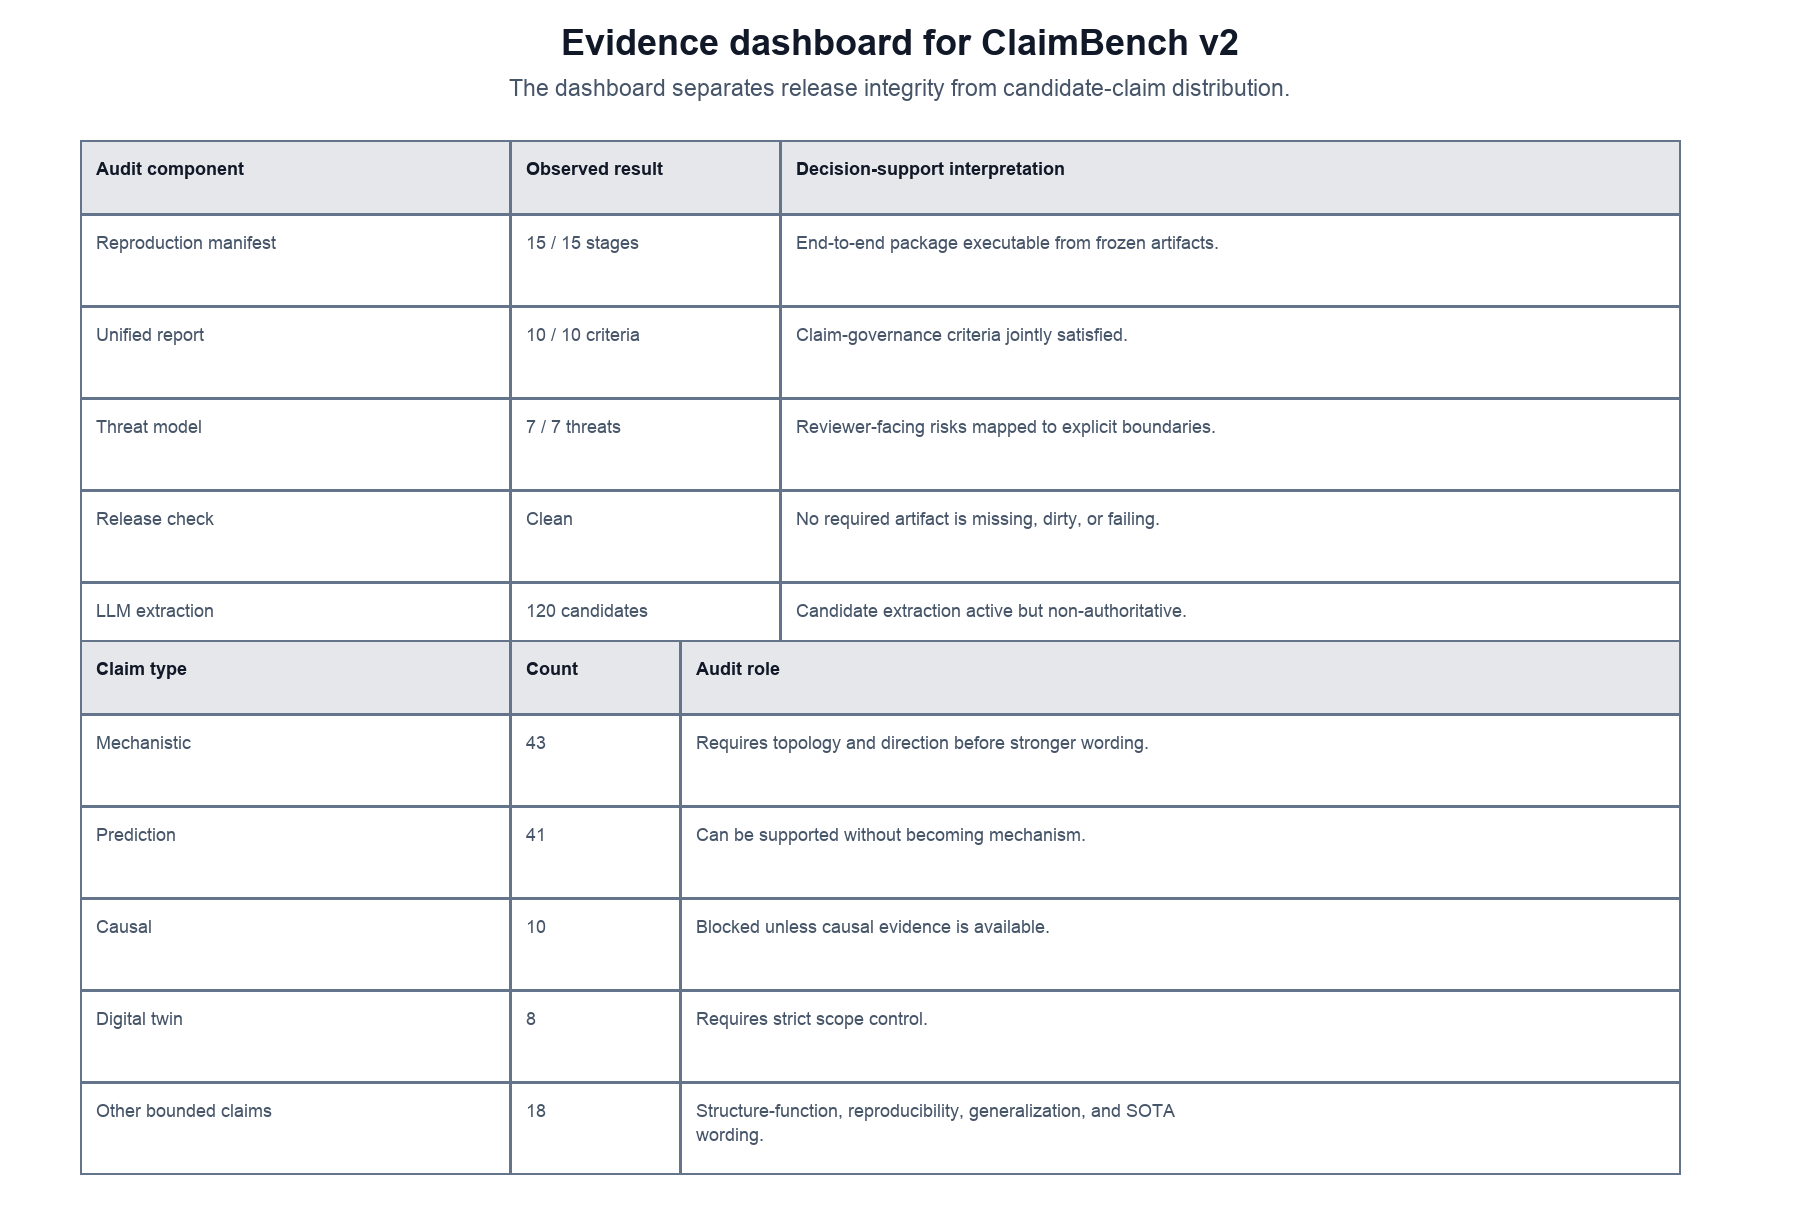
\includegraphics[width=0.94\textwidth]{figures/claimbench_evidence_dashboard.png}
\caption{Frozen release evidence and candidate-claim profile. The upper panel reports engineering integrity checks. The lower panel reports 120 candidates extracted from one revision-specific source corpus. Candidate counts are non-authoritative discovery outputs and do not measure extraction accuracy or constitute an audit of the final submitted manuscript.}
\label{fig:evidence-dashboard}
\end{figure}


For E1, the synthetic known-truth gate evaluates 144 controlled configurations and reports zero claim-gate false positives. This indicates that the non-compensatory rule implements the intended semantics under known evidence states. The important result is not that the synthetic cases are realistic. The important result is that unsupported mechanistic, causal, digital-twin, or state-of-the-art claims are not authorized when the required evidence blocks are absent.

For E2, threshold sensitivity reports both safe and dangerous regions. The unified report records 108 safe settings and 135 dangerous settings. This result is useful because it prevents a misleading threshold narrative. The framework does not claim universal threshold robustness. It reports where the decision is stable and where it would become unsafe. The uncertainty gate also preserves conservative status in borderline cases by blocking unsupported support and keeping unstable supported cases visible.

\begin{table}[t]
\centering
\caption{Summary of the current ClaimBench v2 release artifacts. The table reports the evidence available for the methodological claim and the bounded interpretation assigned by the framework.}
\label{tab:results-summary}
\small
\begin{tabularx}{\textwidth}{p{0.30\textwidth}p{0.22\textwidth}X}
\toprule
Artifact group & Observed result & Bounded interpretation \\
\midrule
Reproduction manifest & 15 of 15 stages passed & End-to-end v2 package is executable from the frozen release \\
Unified report & 10 of 10 criteria passed & Claim-governance criteria are jointly satisfied \\
Threat model & 7 of 7 threats passed & Reviewer-facing risks are mapped to explicit boundaries \\
Release check & 0 missing, 0 dirty, 0 failing & Required artifacts are clean and aligned with expectations \\
Component ablation & 7 high or critical components & Removing core components reintroduces identifiable overclaiming risks \\
LLM claim audit & 120 candidates, non-authoritative & Claim extraction is separated from claim authorization \\
\bottomrule
\end{tabularx}
\end{table}


Fig.~\ref{fig:sensitivity} complements the numerical table by separating three roles that should not be merged. Allen VBN acts as a stable negative case for mechanistic identifiability. Static Sensorium acts as a partial positive case for reliability and topographic organization. Dynamic Sensorium acts as a predictive case with small gains that remain insufficient for mechanistic or causal wording.

\begin{figure}[t!]
\centering
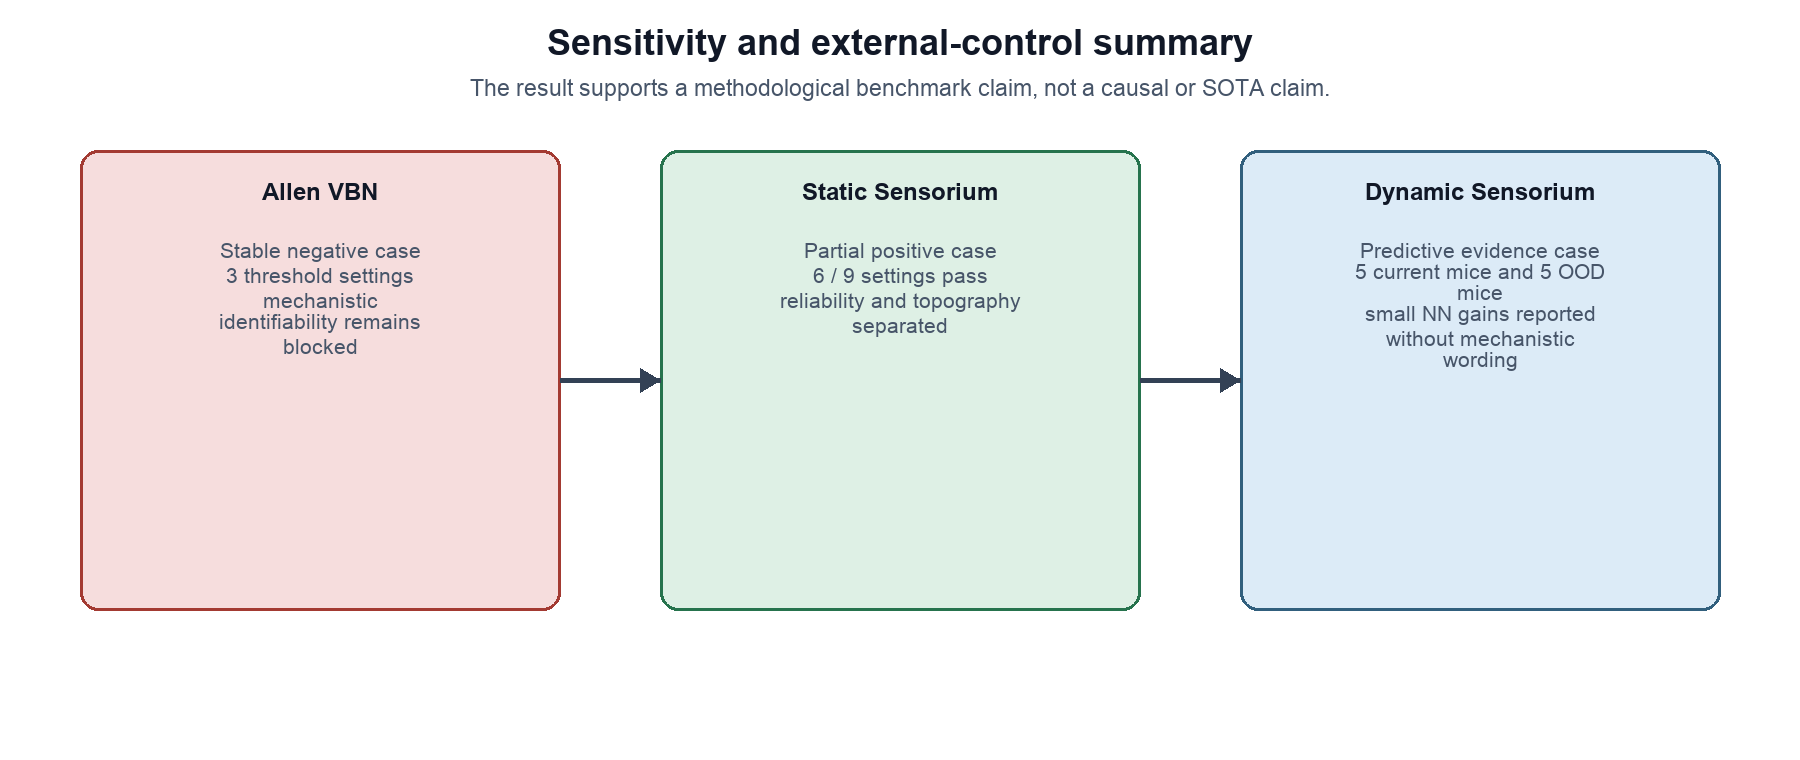
\includegraphics[width=0.94\textwidth]{figures/claimbench_sensitivity.png}
\caption{Sensitivity of the claim gate. Panel A partitions 243 threshold combinations into 108 safe and 135 dangerous cells under the declared criterion. Panel B reports outcomes from deterministic local perturbations of the numerical evidence fields. The resulting stability proportion is an operational robustness measure, not a calibrated probability or confidence interval.}
\label{fig:sensitivity}
\end{figure}


For E3, the SciFact adapter evaluates 300 claims with 124 support labels, 64 contradiction labels, and 112 not-enough-information labels. The transparent BM25 evidence retrieval baseline obtains recall@5 of 0.899. The lexical shortcut produces an overclaiming risk of 0.199, while the BM25-rationale configuration reports an overclaiming risk of 0.250 and a confidence indicator of 0.492. These values are not presented as competitive SciFact performance. They show that retrieval, rationale support, abstention, and overclaiming risk are different decision variables.

For E4, the Tuebingen cause-effect adapter loads 108 pairs and attempts direction on 103 of them. The aggregate direction accuracy is 0.485 and the weighted accuracy is 0.544. This is not sufficient for a causal-discovery performance claim. The useful result is the causal-overclaiming control: 79 correlation-only direction overclaims are identified. The artifact therefore supports the claim that causal wording must remain blocked when direction is not identified.

For E5, the LLM claim extraction audit runs in deterministic fallback mode with an optional local LLM-output file. It identifies 120 candidate claims: 43 mechanistic candidates, 41 prediction candidates, 10 causal candidates, 8 digital-twin candidates, 7 structure-function candidates, 6 reproducibility candidates, 3 generalization candidates, and 2 state-of-the-art candidates. The key result is the boundary condition. No LLM API was called, no LLM candidate was authoritative, and unsupported positive suggestions were not admitted as evidence.

For E6, component ablation identifies eight components and classifies seven as high or critical. Replacing the non-compensatory gate with correlation-only evaluation produces an overclaiming risk of 0.521. Replacing it with a compensatory weighted score produces an overclaiming risk of 0.135. Removing topology or direction blocks allows mechanistic wording to pass when required evidence is absent. Removing causal abstention allows correlation to authorize causal direction. Removing manuscript audit removes the direct link between written claims and executable contracts.

\begin{figure}[t!]
\centering
\resizebox{\textwidth}{!}{%
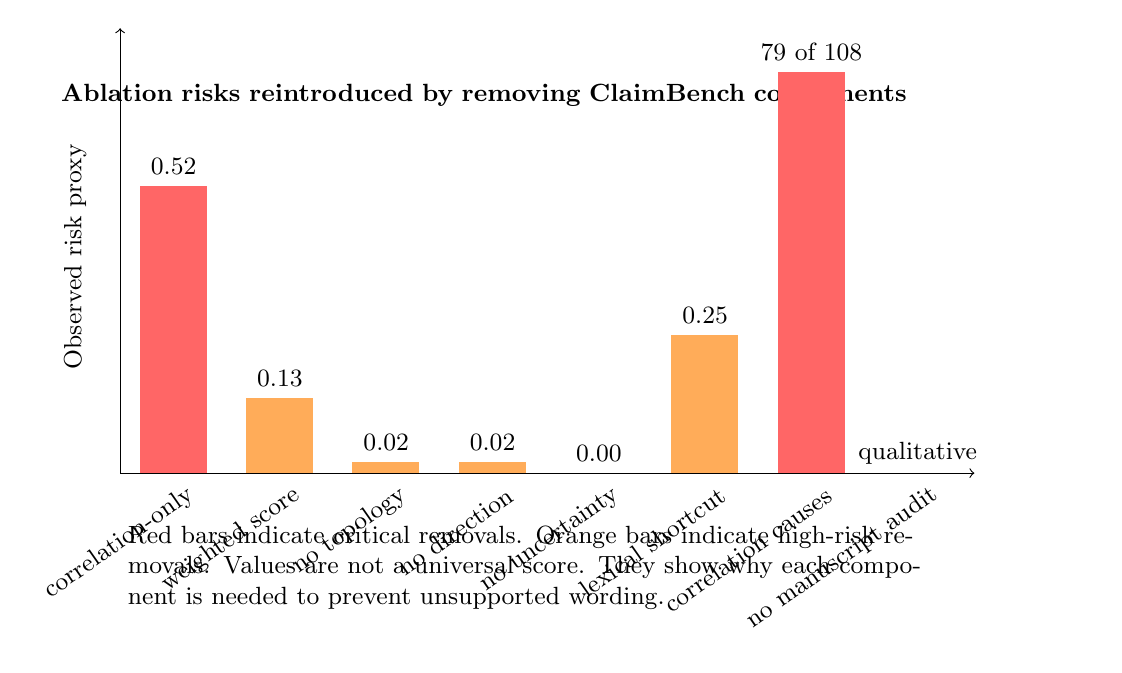
\begin{tikzpicture}[font=\small]
\node[align=left, text width=13cm] at (5.5,4.8) {\textbf{Ablation risks reintroduced by removing ClaimBench components}};
\foreach \x/\h/\lab/\val/\col in {
0/3.65/correlation-only/0.52/red!60,
1.35/0.95/weighted score/0.13/orange!65,
2.7/0.14/no topology/0.02/orange!65,
4.05/0.14/no direction/0.02/orange!65,
5.4/0.0/no uncertainty/0.00/gray!60,
6.75/1.75/lexical shortcut/0.25/orange!65,
8.1/5.1/correlation causes/79 of 108/red!60,
9.45/0.0/no manuscript audit/qualitative/orange!65}
{
  \fill[\col] (\x,0) rectangle +(0.85,\h);
  \node[rotate=35, anchor=east] at (\x+0.75,-0.18) {\lab};
  \node at (\x+0.43,\h+0.25) {\val};
}
\draw[->] (-0.25,0) -- (10.6,0);
\draw[->] (-0.25,0) -- (-0.25,5.65);
\node[rotate=90] at (-0.82,2.75) {Observed risk proxy};
\node[align=left, text width=10.5cm] at (5.1,-1.2) {
Red bars indicate critical removals. Orange bars indicate high-risk removals. Values are not a universal score. They show why each component is needed to prevent unsupported wording.
};
\end{tikzpicture}%
}
\caption{Component ablation summary. Removing non-compensatory gating, causal abstention, or evidence separation reintroduces overclaiming risks that would be hidden by ordinary predictive evaluation.}
\label{fig:ablation}
\end{figure}


For E7, the v2 reproduction package passes all required stages. The manifest reports 15 passed stages out of 15. The unified report passes 10 of 10 criteria. The reviewer threat model passes 7 of 7 tracked threats with no failed critical threat. The release check reports no missing artifacts, no dirty artifacts, and no failing artifacts. Together, these results show that the package is not only conceptually specified, but also inspectable as a release artifact.

The combined result is deliberately bounded. ClaimBench v2 supports a methodological claim about decision support for scientific AI claim governance. It does not support a state-of-the-art SciFact claim, a causal-discovery claim, a new predictive benchmark claim, or a complete digital-twin claim. This negative boundary is part of the result because it demonstrates that the framework blocks the same type of overclaiming that it is designed to audit.
